\documentclass[]{article}
\usepackage[polish]{babel}
\usepackage[cp1250]{inputenc}
\usepackage{polski}
\usepackage[T1]{fontenc}
\frenchspacing
\usepackage{setspace}
\onehalfspacing
\usepackage{indentfirst}
\usepackage{graphicx}
\usepackage{float}

\author{Piotr Turek}

\begin{document}

\begin{figure}
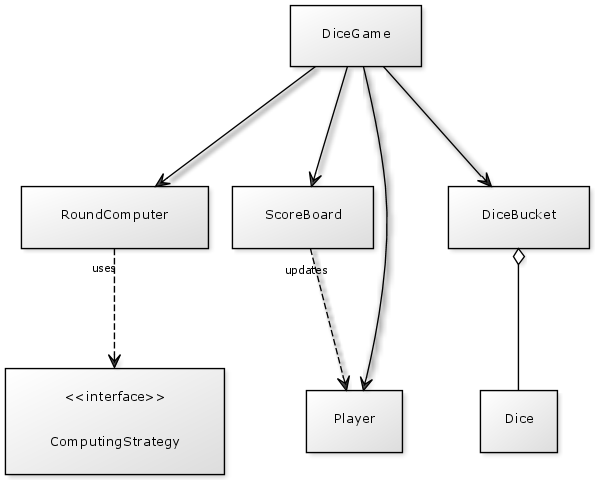
\includegraphics[width=\textwidth]{./diagram.png}
\end{figure}

\section{Komentarz}

\paragraph{}
Klasa \emph{DiceGame} odpowiada za logik� interakcji z u�ytkownikiem. Logik� gry oddelegowuje ona do klasy \emph{RoundComputer}, kt�ra z u�yciem odpowiednich strategii (\emph{ComputingStrategy}) wylicza punktacj� poszczeg�lnych ruch�w. Klasa \emph{ScoreBoard} enkapsuluje aktualny stan gry (wyniki). \emph{DiceBucket} natomiast modeluje kube�ek z kostkami i wszystkie jego funkcjonalno�ci.


\end{document}
